% This is the file where my Master Thesis will be written. It uses the adapted
% LNCS Template.
%
% I'll be using a few codes in the comments, which can be easily looked up:
% * NOTE: theseis-text related comments
% * TODO: thesis-related TODO's
% * WARN: latex/formatting-related warningss
%
% WARN: for running head, subsititute the line below by:
% \documentclass[runningheads,a4paper]{llncs}
\documentclass{llncs}

\usepackage[justification=justified]{caption}
\usepackage{geometry}

%\usepackage[group-separator={,}]{siunitx}k
\usepackage{numprint}

\geometry{
a4paper,         % or letterpaper
textwidth=13.7cm,  % llncs has 12.2cm
textheight=20.4cm, % llncs has 19.3cm
heightrounded,   % integer number of lines
hratio=1:1,      % horizontally centered
vratio=2:3,      % not vertically centered
}
%
%%% WARN: custom extension
%\usepackage{xcolor}
\usepackage[table,xcdraw]{xcolor}
\usepackage{multirow}
\usepackage[normalem]{ulem}
\useunder{\uline}{\ul}{}
\newcommand{\todo}[1]{\textcolor{red}{TODO: #1}\PackageWarning{TODO:}{#1!}}
%%% GLOSSARIES
\usepackage{glossaries}

%%% inline code
\usepackage{xparse}
\NewDocumentCommand{\codeword}{v}{%
\texttt{\textcolor{blue}{#1}}%
}

%%% figures
\usepackage{graphicx}
\usepackage{wrapfig}

%%% tables
\usepackage{booktabs}

\usepackage{amssymb}

\usepackage{url}
\def\UrlBreaks{\do\/\do-}


\makeglossaries

\newacronym{tls}{TLS}{Transport Layer Security}%
\newacronym{ssl}{SSL}{Secure Sockets Layer}%
\newacronym{ietf}{IETF}{Internet Engineering Task Force}%
\newacronym{mac}{MAC}{Message Authentication Code}%
\newacronym{psk}{PSK}{Pre-Shared Key}%
\newacronym{rpk}{RPK}{Raw Public Key}%
\newacronym{aead}{AEAD}{Authenticated Encryption With Associated Data}%
\newacronym{pkc}{PKC}{Public Key Cryptography}%
\newacronym{hmac}{HMAC}{Hash-Based Messaage Authentication Code}%
\newacronym{hkdf}{HKDF}{HMAC-based Extract-and-Expand Key Derivation Function}%
                             \newacronym{html}{HTML}{Hypertext Markup Language}%
\newacronym{https}{HTTPS}{Hypertext Transfer Protocol Secure}%
\newacronym{ecc}{ECC}{Elliptic Curve Cryptography}%
\newacronym{iv}{IV}{Initialization Vector}%
\newacronym{ecdh}{ECDH}{Elliptic Curve Diffie-Hellman}%
\newacronym{ecdhe}{ECDHE}{Elliptic Curve Diffie-Hellman Ephemeral}%
\newacronym{ecdsa}{ECDSA}{Elliptic Curve Digital Signature Algorithm}%
\newacronym{rfc}{RFC}{Request For Comment}%
\newacronym{prf}{PRF}{Pseudo-Random Function}%
\newacronym{rsa}{RSA}{Rivest-Shamir-Adleman}%
\newacronym{dh}{DH}{Diffie-Hellman}%
\newacronym{pms}{PMS}{premaster secret}%
\newacronym{dsa}{DSA}{Digital Signature Algorithm}%
\newacronym{pfs}{PFS}{Perfect Forward Secrecy}%
\newacronym{mitm}{MITM}{Man In The Middle}%
\newacronym{ac}{AC}{Asymmetrical Cryptography}%
\newacronym{sc}{SC}{Symmetrical Cryptography}%
\newacronym{iot}{IoT}{Internet Of Things}%
\newacronym{dtls}{DTLS}{Datagram TLS}%
\newacronym{tlsd}{(D)TLS}{(D)TLS}%
\newacronym{coap}{CoAP}{Constrained Application Protocol}%
\newacronym{ec}{EC}{Elliptic Curve}%
\newacronym{sca}{SCA}{Side-Channel Attack}%
\newacronym{ocsp}{OCSP}{Online Certificate Status Protocol}
\newacronym{crl}{CRL}{Certificate Revocation List}
\newacronym{ca}{CA}{Certification Authority}
\newacronym{sni}{SNI}{Server Name Indication}
\newacronym{dos}{DoS}{Denial-of-Service}
\newacronym{ddos}{DDoS}{Distributed Denial-Of-Service}
\newacronym{pki}{PKI}{Public Key Infrastructure}
\newacronym{ae}{AE}{Authenticated Encryption}
\newacronym{nsa}{NSA}{US National Security Agency}
\newacronym{apk}{APK}{Authorized Public Key}
\newacronym{iana}{IANA}{Internet Assigned Numbers Authority}
\newacronym{jit}{JIT}{just-in-time}
\newacronym{ir}{IR}{Intermediate Representation}


%%% WARN: added as specified here:
% https://tex.stackexchange.com/questions/272200/table-of-contents-showing-the-title-as-only-entry-latex
\setcounter{tocdepth}{2}
\makeatletter
\renewcommand*\l@author[2]{} % removes author name from TOC
\renewcommand*\l@title[2]{} % removes title name from TOC
\makeatletter
%%%
%
\usepackage{makeidx}  % allows for indexgeneration
%
\newcounter{footnotesintable}
%
\begin{document}
%
\frontmatter          % for the preliminaries
%
\pagestyle{headings}  % switches on printing of running heads
%
\addtocmark{TLS For IoT} % additional mark in the TOC

\tableofcontents
\newpage

\mainmatter              % start of the contributions
%
\title{Transport Layer Security Protocol For Internet Of Things Extended Abstract}
%
\titlerunning{TLS For IoT}  % abbreviated title (for running head)
%                                     also used for the TOC unless
%                                     \toctitle is used
%
\author{{Illya Gerasymchuk} \\
\email{illya@iluxonchik.me}}
%
\authorrunning{Illya Gerasymchuk} % abbreviated author list (for running head)
%
%%%% list of authors for the TOC (use if author list has to be modified)
\tocauthor{Illya Gerasymchuk}
%
\institute{Instituto Superior Tecnico}
% WARN: supper hacked-in
\supervisors{Ricardo Chaves, Aleksandar Ilic}
\maketitle              % typeset the title of the contribution

\begin{abstract}
\gls{tls} is one of the most used communication security protocols in the world. It comes with many configurations. 
Each configuration offers a set o security services, which has an implication on the 
security level and computational cost.
Not all of those configurations can be used with the resource constrained \gls{iot} devices, due to the
high computational and memory demands. Most of the existing work focuses on \gls{dtls}
and cannot be easily integrated with existing deployments. Existing work fails
to evaluate the cost of various \gls{tls} configurations and its security services.
This work focuses on cost analysis of the security services of the TLS protocol.
We evaluate the number of CPU cycles used by the TLS configurations
and by each individual security service. Software developers can use this information
to make security/cost trade-offs based on the environment needs and limitations.  

\keywords{TLS, DTLS, SSL, IoT, cryptography, protocol, lightweight cryptography}
\end{abstract}
%
\section{Introduction}
%

In recent years there has been a sharp increase in the number of IoT
devices and this trend is expected to continue. The IoT is a network
of interconnected devices, which exchange data with one another over
the internet. While they are many types of IoT devices, all of them
are restricted: they have limited memory, processing power and
available energy. Examples of IoT devices include temperature sensors,
smart light bulb and physical activity trackers.

While inter-device communication has numerous benefits, it is important
to ensure the security of that communication. For example, when you log
in to your online banking account, you do not want others to be
able to see your password, as this may lead to the compromise of your
account. Having your account compromised means that a malicious entity
might steal your money. Similarly, when you are transferring funds via
online banking, you want the contents of that operation to be
invisible to an observer, for privacy reasons. It is also desirable
that no party is able to tamper with the transmitted data en transit,
as it may lead to undesired consequences, such as the transfer of a
larger amount than you intended. Proper communications security allows
those goals to be achieved.

\gls{tls} is one of the most used protocols for communication security. It
powers numerous technologies, such as \gls{https}. TLS offers the
security services of authentication, confidentiality, privacy, integrity, replay
protection and perfect forward secrecy. It is not a requirement to use all of
those services for every TLS connection. The protocol is similar to
a framework, in the sense that you can enable individual security
services on a per-connection basis. For example, when you are downloading
software updates, data confidentiality is probably not a concern,
data authenticity and integrity, however, is. In TLS, it is possible for a connection
to only offer authenticity and integrity, without offering confidentiality.
Foregoing unnecessary services will lead to a smaller resource usage,
which in turn leads to smaller execution time and power usage. This
is especially important in the context of IoT, due to the constrained
nature of the devices.

There are numerous IoT devices, each one with different hardware
capabilities and security requirements. For example, some IoT
devices have the capability of using public key cryptography,
while for others symmetric cryptography is the only option
In some cases, the communicating devices require data authenticity, confidentiality
and integrity (e.g. when logging in into a device), while in others data
authenticity and integrity is enough (e.g. when transferring updates).

TLS was not designed for the constrained environment of IoT. Despite that,
it is a malleable protocol and can be configured to one's needs. In essence,
it is a combination of various security algorithms that together form
a protocol for communication security. If configured
properly, it is possible to use it in the context of IoT. Existing work
does not address the computational cost evaluation of the various security services
offered by TLS individually. An example of a computational is the number of CPU
cycles used, time taken or power used. Thus, software developers
who want to use TLS to provide connection security do not have data that can
assist them in making the security/resource usage trade-offs

The goal of this work is to evaluate the cost of each security service of the
TLS protocol. This will assist software developers to make security/resource usage
trade-off judgments, according to their needs and limitations. For this reason,
this work targeted towards developers who wish to add communication security
to their applications in the IoT environment.

In the process of the work on this dissertation, we have made several
contributions to the \gls{tls} $1.3$ specification, and were formally recognized as 
contributors\cite{Mergepul65:online}. Our name can be found in the document specifying \gls{tls} $1.3$\cite{RFC8446}.
We have also found a security issue within the
\gls{tls} implementation of the \textit{mbedTLS} library. We reported it and it
has been assigned a \textit{CVE} with the id \textit{CVE-2018-1000520}\cite{NVDCVE2094:online}.
It is an authentication problem, where certificates signed with an incorrect algorithm
were accepted in some cases. More specifically, \textit{ECDH(E)-RSA} ciphersuites allowed \gls{ecdsa}-signed
certificates, when only \gls{rsa}-signed ones should be. We also found a bug in \textit{mbedTLS}'s test suite
related to the use of deprecated \textit{SHA-1}-signed certificates and submitted a code fix to 
it \cite{sslserve89:onelin}\cite{updatete23:online}.

\section{Motivation}

The majority of existing work on \gls{tlsd} optimization proposes 
a solution that is either tied to a
specific protocol, such as \gls{coap}, or requires an introduction of a third-party
entity, such as the trust anchor in the case of the S3K system\cite{S3KScala62:online} or
even both. This has two issues. First, a protocol-specific solution cannot
be easily used in an environment where (D)\gls{tls} is not used with that protocol.
Second, the requirement of a third-party
introduces additional cost and complexity, which will be a big resistance factor
in adopting the technology. This is specially true for developers working on
personal projects or projects for small businesses, leaving the communications insecure
in the worse case scenario. Therefore a solution that is protocol independent and fully 
compatible with the \gls{tlsd} standard and existing infrastructure is desired.

Another issue with the existing literature is that it almost exclusively focuses on \gls{dtls} optimization
and not all of it can be applied to \gls{tls}. Herein we want to further explore \gls{tls} optimization. 
There is clearly a need for that,
specially with \gls{coap} over TCP and \gls{tls} standard being currently developed. The
mentioned standard does not explore any \gls{tls} optimizations, and since any
\gls{iot} device using it in the future would benefit from them, this is an important
area to explore.

(D)\gls{tls} is a complex protocol with numerous possible configurations. Each configuration
provides different set security services and a different security level. This has a direct
impact on the resource usage. Thus, the cost of a \gls{tlsd} connection can be lowered,
by using an appropriate configuration. Typically, this involves making security/cost trade-offs.
Optimizing the connection cost in this way meets our goals of being protocol independent, fully compatible with
existing infrastructure and targeting \gls{tls} optimization specifically.

The objective of this work is to provide a means of assisting application developers
who wish to include secure communications in their applications to make
security level/resource usage trade-offs, according to the environment's needs
and limitations. In order to achieve this goal, the costs of each individual security service
will be evaluated. With this information, the programer will be able to choose a configuration that
meets his security requirements and device constraints. If the limitations of the device's hardware
do not allow to meet the requirements, the programer may decide on an alternative configuration, possibly with
a loss of some security services and a lower security level, or forgo using (D)\gls{tls} altogether.

\section{Methodology}

In our work, we evaluated the \textit{mbedTLS's} implementation of the \gls{tls} protocol, thus obtained
metrics reflect the algorithm's implementations used within the library. The metric that we evaluated is the number
of CPU cycles executed. To be more precise, an estimate of that value. 
In order to estimate the number of executed cycles, we used \textit{valgrind}, more specifically
its \textit{callgrind} tool. \textit{valgrind} runs the application on a synthetic CPU.
While running the code in that synthetic environment, it is able to insert instructions to perform
profiling and debugging. In essence, \textit{valgrind} is a virtual machine, using \gls{jit}
compilation techniques, such as dynamic recompilation.

Among other metrics, \textit{callgrind}
collects the number of executed instructions, L1/L2 caches misses (the caches are simulated), and branch
prediction misses. The metrics collected by \textit{callgrind} can then be loaded into \textit{kcachegrind}
to visualize and analyze the performance results. One of such results is the estimate of the number of executed CPU cycles.
\textit{callgrind} and \textit{kcachegrind} are widely in conjunction for performance analysis and optimization
of programs. In order to count the number of executed CPU cycles, we used the following formula (derived from the one used by \textit{kcachegrind}): $CEst = Ir + 10*Bm + 10*L1m + 100*L2m$,
where $Ir$ is the number of instruction fetches, $Bm$ is the number of mispredicted branches and $L1m$ and $L2m$ are the number
L1 and L2 cache misses, respectively.

In order to estimate the number of CPU cycles, we developed automated tooling that collected and analyzed the metrics output by
\textit{callgrind}. All of the evaluations were performed in
our local \textit{Intel(R) Core(TM) i7-4700HQ} machine.

\section{Evaluation}

The \gls{tlsd} protocol consists of two sub-protocols: the Handshake protocol and the Record protocol.
During the Handshake protocol, the peers authenticate one to another, agree on the data encryption and integrity
algorithms and establish the shared keys. It offers the security services of confidentiality and integrity. 
During the Record protocol the peers exchange the data securely, using the algorithms and keys 
negotiated during the Handshake protocol. Those algorithms support the security services provided by \gls{tlsd}.

The core of the Record protocol is the use of a symmetric encryption algorithm (\textit{e.g} AES), used to
provide confidentiality and an \gls{hmac} algorithm, used to provide data integrity and data origin authentication.
The performance of symmetric encryption
algorithms and hash functions has been studied in detail by existing work \cite{nadeem2005performance} \cite{mathew2010performance}.
There is an approximately linear relation between the amount of data encrypted and the the cost.

The previous paragraph does not apply to the Handshake protocol. In this part, there is more variety in the
computational cost outcomes. There are a few reasons for that. First, there are significantly more possible key sizes (unlimited, in theory), when compared to
symmetric encryption algorithms. Second, various algorithms, in various combinations can be used to provide 
authentication and \gls{pfs}. Third, the use of asymmetric cryptography leads to asymmetric costs (\textit{i.e.} distinct costs) for the client and the server. The costs of asymmetric
encryption algorithms vary greatly depending if the public or the private key is used. 

It is clear that the Handshake protocol is significantly more complex, with more possible cost variations.
Furthermore, existing work neither evaluated the costs of individual security services of \gls{tls}, nor
their various combinations. For this reason, our work is concentrated around the Handshake protocol.

We evaluated the costs for various security services, defined in table \ref{table:tls-sec-lvls}. We analyzed for the most common 
authentication scenario only: only the server authenticates to the client. As a consequence, the costs of authentication
are different for the client and the server.

\begin{table}[]
  \begin{tabular}{|l|l|l|l|l|}
  \hline
                                                                       & \textbf{low} & \textbf{normal} & \textbf{high} & \textbf{very high} \\ \hline
  \begin{tabular}[c]{@{}l@{}}Symmetric Key Size\\ (bits)\end{tabular}  & 128               & 128               & 192\addtocounter{footnote}{1}\addtocounter{footnotesintable}{1}\footnotemark[\thefootnote]             & 256            \\ \hline
  \begin{tabular}[c]{@{}l@{}}RSA/DH/DSA Key Size\\ (bits)\end{tabular} & 1024              & 2048              & 4092          & 8192           \\ \hline
  \begin{tabular}[c]{@{}l@{}}ECC Key Size\\ (bits)\end{tabular}        & 163 \addtocounter{footnote}{1}\addtocounter{footnotesintable}{1} \footnotemark[\thefootnote]               & 233 \addtocounter{footnote}{1}\addtocounter{footnotesintable}{1}\footnotemark[\thefootnote]               & 317\addtocounter{footnote}{1}\addtocounter{footnotesintable}{1}\footnotemark[\thefootnote]             & 420\addtocounter{footnote}{1}\addtocounter{footnotesintable}{1}\footnotemark[\thefootnote]              \\ \hline
  HMAC                                                                 & SHA-256           & SHA-256           & SHA-384       & SHA-512  \addtocounter{footnote}{1}\addtocounter{footnotesintable}{1}\footnotemark[\thefootnote]      \\ \hline
  \end{tabular}
  \centering \caption{\label{table:tls-sec-lvls} Security levels used in evaluation}
  \end{table}

\addtocounter{footnote}{-\thefootnotesintable}
\addtocounter{footnote}{1}\footnotetext[\thefootnote]{The closest value available in mbedTLS 2.7.0 (rounded up) is $256$ bit}
\addtocounter{footnote}{1}\footnotetext[\thefootnote]{The closest value available in mbedTLS 2.7.0 (rounded up) is $224$ bit}
\addtocounter{footnote}{1}\footnotetext[\thefootnote]{The closest value available in mbedTLS 2.7.0 (rounded up)is $256$ bit}
\addtocounter{footnote}{1}\footnotetext[\thefootnote]{The closest value available in mbedTLS 2.7.0 (rounded up) is $384$ bit}
\addtocounter{footnote}{1}\footnotetext[\thefootnote]{The closest value available in mbedTLS 2.7.0 (rounded up) is $512$ bit}
\addtocounter{footnote}{1}\footnotetext[\thefootnote]{The strongest hash function available in mbedTLS is SHA-384}


\subsection{Authentication Cost Analysis}

In \gls{tls} there are two ways of doing authentication: either by using a \gls{psk} or by using asymmetric cryptography.

If only \gls{psk} is used for authentication (\textit{PSK} key exchange), the cost of authentication is practically $0$. In this case, the
peers perform the simplest handshake available in \textit{mbedTLS 2.7.0}. The cost of a handshake that uses
the \textit{PSK} can be considered as the overhead of establishing the \gls{tls} connection.

If asymmetric cryptography is used for authentication, there are two
choices of algorithms: \gls{rsa} and \gls{ecdsa}. Each one of them has advantages and disadvantages, depending on the
scenario. \gls{rsa} is more efficient at performing public key operations, \textit{i.e.} verifying the signature. \gls{ecdsa} is more efficient at performing private key operations, 
\textit{i.e.} making the signature. Figure \ref{fig:ecdsa-rsa-costs-all}
shows the costs of both, \gls{rsa}'s and \gls{ecdsa}'s operations. The data is presented in logarithmic scale.
The \textit{Total} cost is the sum of the costs of the signature creation and verification operations.
Since for \gls{rsa} most of the \textit{Total} cost comes from the signature creation operation, 
those two lines overlap in the graph.

\begin{figure}
  \centering
  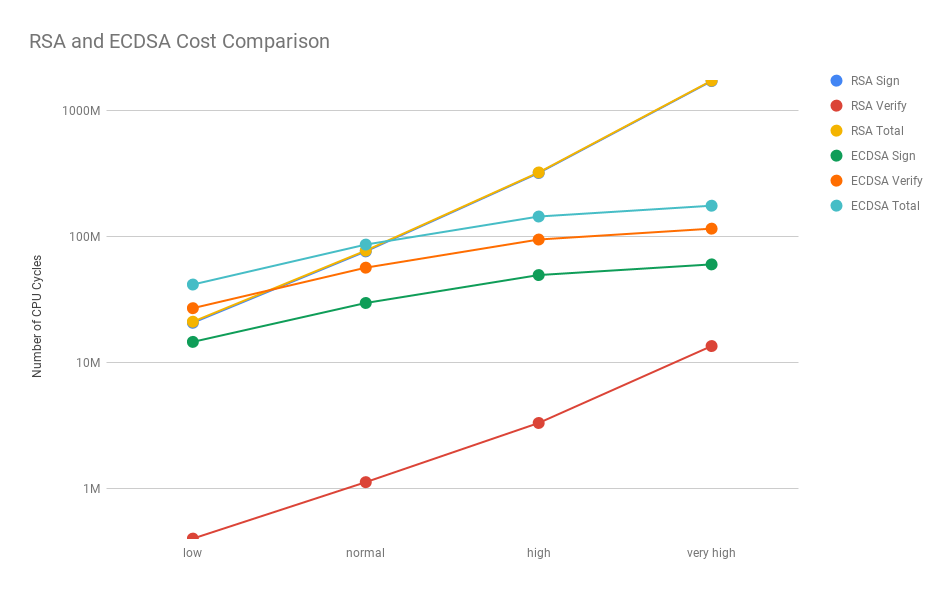
\includegraphics[width=1.0\textwidth]{img/rsa_ecdsa_costs_all.png}
  \centering \caption{\label{fig:ecdsa-rsa-costs-all} RSA and ECDSA cost comparison}
\end{figure}

By analyzing Figure \ref{fig:ecdsa-rsa-costs-all}, we can contrast both of the algorithms. First, while 
\gls{rsa} is always less costly at signature verification, \gls{ecdsa} is always less costly at signature creation,
Second, while \gls{rsa}'s cost increase is exponential,\gls{ecdsa}'s cost increase is logarithmic. 
And finally, while the total cost of \gls{rsa} is smaller for the \textit{low} and \textit{normal} security levels,
the total cost of \gls{ecdsa} is smaller for the \textit{high} and \textit{very high} security levels.

The properties of both algorithms have a direct impact on the \gls{tls} handshake costs. Table \ref{table:tls-auth-cost-client} shows authentication costs for each
ciphersuite for the client. Table \ref{table:tls-auth-cost-server} shows the same information for the server. Each row specifies a key
exchange method and each column the security level.

\begin{table}[]
  \begin{tabular}{|l|l|l|l|l|}
  \hline
                       & \textbf{low} & \textbf{normal} & \textbf{high} & \textbf{very high} \\ \hline
  \textbf{PSK}         & 0            & 0               & 0             & 0                  \\ \hline
  \textbf{RSA}         & 654077       & 2622235         & 5285561       & 16398134           \\ \hline
  \textbf{RSA-PSK}     & 654077       & 2622235         & 5285561       & 16398134           \\ \hline
  \textbf{ECDH-RSA}    & 1117868      & 1117868         & 1117868       & 1117868           \\ \hline
  \textbf{ECDH-ECDSA}  & 56260702     & 56260702        & 56260702      & 56260702          \\ \hline
  \textbf{ECDHE-PSK}   & 0            & 0               & 0             & 0                  \\ \hline
  \textbf{ECDHE-RSA}   & 1516452       & 2235736         & 4413164       & 14554596           \\ \hline
  \textbf{ECDHE-ECDSA} & 83099975     & 112521404       & 150337852     & 171004723          \\ \hline
  \textbf{DHE-PSK}     & 0            & 0               & 0             & 0                  \\ \hline
  \textbf{DHE-RSA}     & 1516452       & 2235736         & 4413164       & 14554596           \\ \hline
  \end{tabular}
  \centering \caption{\label{table:tls-auth-cost-client} Client authentication costs for all ciphersuites and security levels}
  \end{table}

\begin{table}[]
\begin{tabular}{|l|l|l|l|l|}
\hline
                     & \textbf{low} & \textbf{normal} & \textbf{high} & \textbf{very high} \\ \hline
\textbf{PSK}         & 0            & 0               & 0             & 0                  \\ \hline
\textbf{RSA}         & 20362831     & 75129504        & 314975365     & 1691976601         \\ \hline
\textbf{RSA-PSK}     & 20362831     & 75129504        & 314975365     & 1691976601         \\ \hline
\textbf{ECDH-RSA}    & 0            & 0               & 0             & 0                  \\ \hline
\textbf{ECDH-ECDSA}  & 0            & 0               & 0             & 0                  \\ \hline
\textbf{ECDHE-PSK}   & 0            & 0               & 0             & 0                  \\ \hline
\textbf{ECDHE-RSA}   & 20559190     & 75738802        & 317087210     & 1700652764         \\ \hline
\textbf{ECDHE-ECDSA} & 14497591     & 29512991        & 49150396      & 59732056           \\ \hline
\textbf{DHE-PSK}     & 0            & 0               & 0             & 0                  \\ \hline
\textbf{DHE-RSA}     & 20559190     & 75738802        & 317087210     & 1700652764         \\ \hline
\end{tabular}
  \centering \caption{\label{table:tls-auth-cost-server} Server authentication costs for all ciphersuites and security levels}
\end{table}

\subsection{\gls{pfs} Cost Analysis}

In \gls{tls} there are two ways of achieving \gls{pfs}: either by using the \gls{dh} algorithm 
or its \gls{ecc} counterpart \gls{ecdh}.

Figure \ref{fig:ecdh-dh-costs-all} compares the costs of \gls{ecdh} and \gls{dh}. If the \textbf{low} security level is being used,
\gls{dh} is the least costly choice, if the \textbf{normal} or any security level above is being used, \gls{ecdh} is. Moreover, we can clearly see that
for each algorithm, the costs of their operations is very similar, since we have overlapping lines. The logarithmic and exponential properties of
\gls{ecdh} and \gls{dh}, respectively, are also visible by shape of the lines. Since we are using logarithmic scale for the $y$ axis, the
exponential cost growth of \gls{dh} manifests in the shape of a line.

\begin{figure}
  \centering
  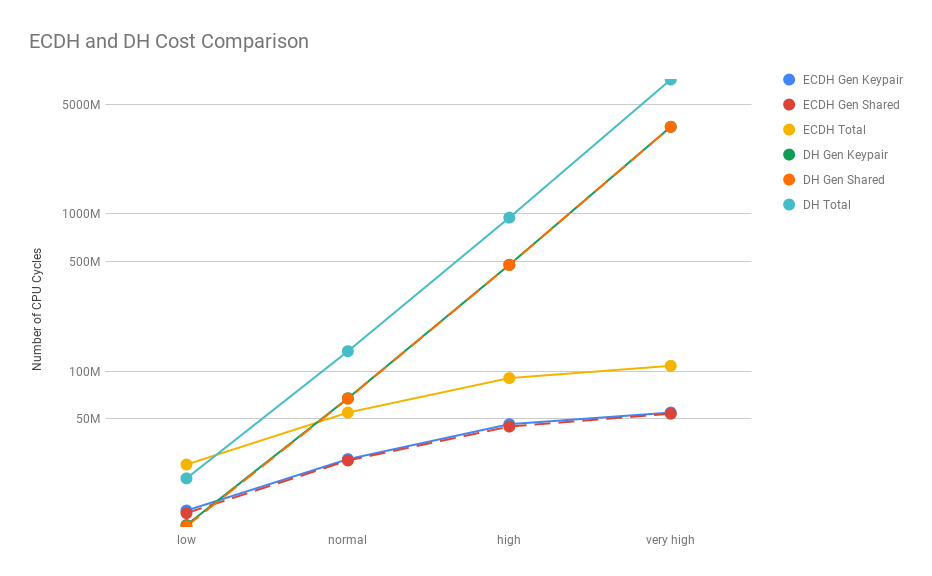
\includegraphics[width=1.0\textwidth]{img/ecdh_dh_costs_all.png}
  \centering \caption{\label{fig:ecdh-dh-costs-all} ECDH and DH cost comparison (logarithmic scale)}
\end{figure}

Even though the \textit{ECDH} key exchange does not offer \gls{pfs}, it is still closely related to the \textit{ECDHE}, since both use
the \gls{ecdh} algorithm. The additional costs for \textit{ECDH} ciphersuites are significant, and in our evaluated scenario where only the server
authenticates to the client, there is no distinction in costs between \textit{ECDHE} and \textit{ECDH} ciphersuites for the client. 
Tables \ref{table:pfs-cost-client} and \ref{table:pfs-cost-server} show the cost of \gls{pfs} and the \textit{ECDH} key exchanges for the client and the server, respectively.

\begin{table}[]
\begin{tabular}{|l|l|l|l|l|}
\hline
                                           & \textbf{low}                    & \textbf{normal}                 & \textbf{high}                   & \textbf{very high}               \\ \hline
\textbf{PSK}                               & 0                               & 0                               & 0                               & 0                                \\ \hline
\textbf{RSA-PSK}                           & 0                               & 0                               & 0                               & 0                                \\ \hline
\textbf{RSA}                               & 0                               & 0                               & 0                               & 0                                \\ \hline
\rowcolor[HTML]{9B9B9B}
{\color[HTML]{333333} \textbf{ECDH-RSA}}   & {\color[HTML]{333333} 25405195} & {\color[HTML]{333333} 54442524} & {\color[HTML]{333333} 90231688} & {\color[HTML]{333333} 107981294} \\ \hline
\rowcolor[HTML]{9B9B9B}
{\color[HTML]{333333} \textbf{ECDH-ECDSA}} & {\color[HTML]{333333} 25405195} & {\color[HTML]{333333} 54442524} & {\color[HTML]{333333} 90231688} & {\color[HTML]{333333} 107981294} \\ \hline
\textbf{ECDHE-PSK}                         & 25405195                        & 54442524                        & 90231688                        & 107981294                        \\ \hline
\textbf{ECDHE-RSA}                         & 25405195                        & 54442524                        & 90231688                        & 107981294                        \\ \hline
\textbf{ECDHE-ECDSA}                       & 25405195                        & 54442524                        & 90231688                        & 107981294                        \\ \hline
\textbf{DHE-PSK}                           & 20734678                        & 133849027                       & 948573054                        & 7178955325                        \\ \hline
\textbf{DHE-RSA}                           & 25405195                        & 133849027                        & 948573054                        & 7178955325                        \\ \hline
\end{tabular}
\centering \caption{\label{table:pfs-cost-client} \gls{pfs} and \textit{ECDH} key exchange for the client}
\end{table}

\begin{table}[]
\begin{tabular}{|l|l|l|l|l|}
\hline
                                           & \textbf{low}                    & \textbf{normal}                 & \textbf{high}                   & \textbf{very high}              \\ \hline
\textbf{PSK}                               & 0                               & 0                               & 0                               & 0                               \\ \hline
\textbf{RSA-PSK}                           & 0                               & 0                               & 0                               & 0                               \\ \hline
\textbf{RSA}                               & 0                               & 0                               & 0                               & 0                               \\ \hline
\rowcolor[HTML]{9B9B9B}
{\color[HTML]{333333} \textbf{ECDH-RSA}}   & {\color[HTML]{333333} 12462677} & {\color[HTML]{333333} 26958612} & {\color[HTML]{333333} 44331330} & {\color[HTML]{333333} 53531554} \\ \hline
\rowcolor[HTML]{9B9B9B}
{\color[HTML]{333333} \textbf{ECDH-ECDSA}} & {\color[HTML]{333333} 12462677} & {\color[HTML]{333333} 26958612} & {\color[HTML]{333333} 44331330} & {\color[HTML]{333333} 53531554} \\ \hline
\textbf{ECDHE-PSK}                         & 25405195                        & 54442524                        & 90231688                        & 107981294                       \\ \hline
\textbf{ECDHE-RSA}                         & 25405195                        & 54442524                        & 90231688                        & 107981294                       \\ \hline
\textbf{ECDHE-ECDSA}                       & 25405195                        & 54442524                        & 90231688                        & 107981294                       \\ \hline
\textbf{DHE-PSK}                           & 20734678                        & 133849027                       & 948573054                        & 7178955325                       \\ \hline
\textbf{DHE-RSA}                           & 20734678                        & 133849027                       & 948573054                        & 7178955325                       \\ \hline
\end{tabular}
\centering \caption{\label{table:pfs-cost-server} \gls{pfs} and \textit{ECDH} key exchange for the server}
\end{table}

\subsection{Handshake Cost Analysis}

Having analysed the cost of the security services of authentication and \gls{pfs}, we are now ready to analyze the cost of the handshake.
Tables \ref{table:client-hs-cost-all-sls} and \ref{table:server-hs-cost-all-sls} show the average handshake cost for each one of the
key exchange methods, for the client and server, respectively. We can use the following formula to compute the cost of the \gls{tls} Handshake cost for a key exchange method and
security level: $Handshake Cost = TLS Overhead + Auth Cost + PFS Cost + Additional Costs$. The \textit{TLS Overhead} is the cost of the
\textit{PSK} key exchange and can be obtained from table \ref{table:client-hs-cost-all-sls} for the client
and from table \ref{table:server-hs-cost-all-sls} for the server. \textit{Auth Cost} is the cost of authentication and can be obtained
from \ref{table:tls-auth-cost-client} for the client and from table \ref{table:tls-auth-cost-server} for the server. \textit{PFS} cost
is the cost of \gls{pfs} and can be obtained from table \ref{table:pfs-cost-client} for the client and from table \ref{table:pfs-cost-server}
for the server. \textit{Additional Costs} come from the \textit{Certificate} message.
This message is omitted entirely in the \textit{PSK} key exchange. In ciphersuites that use asymmetric authentication,
the client has to read the  \textit{Certificate} message from the record layer, parse the \textit{der} encoded certificate into internal fields and
check the validity of its fields, such as the not valid before/after dates. The server has to write the \textit{Certificate} message to the
record layer. This cost for the client is approximately $622615$.

As an example, we will compute the client's Handshake cost for the \textbf{high} security level with \textit{ECHDE-RSA}
First, we will need to get the \textit{TLSOverhead} value. We can obtain in from the entry located at the
\textit{ECDHE-RSA} row and \textit{high} column in table \ref{table:client-hs-cost-all-sls}: $1355005$. \textit{AuthCost} can be obtained
from the \textit{ECDHE-RSA} row and \textit{high} column in table \ref{table:tls-auth-cost-client}: $4413164$. Similarly \textit{PFSCost}
can be obtained from table \ref{table:pfs-cost-client}, where the \textit{ECDHE-RSA} row and \textit{high} column intersect: $90231688$.
The $AdditionalCosts$ value is $622615$. All that's left now is insert those values in the formula:
$Handshake Cost = TLS Overhead + Auth Cost + PFS Cost + Additional Costs = 1355005 + 4413164 + 90231688 + 622615 = 96622472$.
As we can see, the cost computed using the formula is very close to the actual Handshake cost when evaluated as a whole,
which can be found in in table \ref{table:client-hs-cost-all-sls}. The difference of $108429$ ($96730901-96607399$) CPU cycles comes 
from other additional costs, such as reading and writing slightly larger messages.

\begin{table}[]
  \begin{tabular}{|l|l|l|l|l|}
  \hline
                       & \textbf{low}      & \textbf{normal}    & \textbf{high}      & \textbf{very high}   \\ \hline
  \textbf{PSK}         & 1354543    & 1353865     & 1355005     & 1354829       \\ \hline
  \textbf{RSA-PSK}     & 3536763     & 4543238      & 7293473      & 18578392      \\ \hline
  \textbf{RSA}         & 3556430     & 4558935      & 7309587      & 18608492       \\ \hline
  \textbf{ECDH-RSA}    & 28433250    & 57412269    & 93325335    & 111532116     \\ \hline
  \textbf{ECDH-ECDSA}  & 83731926    & 112585306   & 148415289   & 166815336     \\ \hline
  \textbf{ECDHE-PSK}   & 26819362    & 55805138    & 91713096    & 109203285     \\ \hline
  \textbf{ECDHE-RSA}   & 28862986   & 58608367    & 96730901     & 124773055     \\ \hline
  \textbf{ECDHE-ECDSA} & 110524836   & 168954007   & 242501399   & 280626510    \\ \hline
  \textbf{DHE-PSK}     & 22189619    & 135442518   & 950212732   & 7181764421   \\ \hline
  \textbf{DHE-RSA}     & 24250886    & 138197524   & 955840114   & 7196088947   \\ \hline
  \end{tabular}
  \centering \caption{\label{table:client-hs-cost-all-sls} Handshake costs for the client}
  \end{table}

  \begin{table}[]
\begin{tabular}{|l|l|l|l|l|}
\hline
                     & \textbf{low}      & \textbf{normal}    & \textbf{high}       & \textbf{very high}   \\ \hline
\textbf{PSK}         & 1380956     & 1382849      & 1381497       & 1382002        \\ \hline
\textbf{RSA-PSK}     & 22515609   & 77368868    & 317389619    & 1694178055   \\ \hline
\textbf{RSA}         & 22456180   & 77260738    & 317196961    & 1694747500   \\ \hline
\textbf{ECDH-RSA}    & 14534087    & 29154666    & 46480720     & 55636527      \\ \hline
\textbf{ECDH-ECDSA}  & 14521154    & 29094320    & 46390603     & 55927921      \\ \hline
\textbf{ECDHE-PSK}   & 26869449   & 56020895    & 91773474      & 109500050     \\ \hline
\textbf{ECDHE-RSA}   & 48164890   & 132433386   & 409652623    & 1810563620   \\ \hline
\textbf{ECDHE-ECDSA} & 41984222    & 86096716    & 141506181    & 169996896    \\ \hline
\textbf{DHE-PSK}     & 22308029    & 135535409   & 950691653   & 7181243788   \\ \hline
\textbf{DHE-RSA}     & 43602094   & 212251542   & 1268235354   & 8883866054   \\ \hline
\end{tabular}
  \centering \centering \caption{\label{table:server-hs-cost-all-sls} Handshake costs for the server}
\end{table}

\subsection{Confidentiality Cost Analysis}

Our evaluation of the encryption algorithms in \textit{mbedTLS 2.7.0} showed that \textit{3DES} is the most costly one of all, 
while \gls{aead} encryption algorithms 
(\textit{AES} with \textit{GCM} and \textit{CCM} modes) are the least costly block cipher algorithms. 
\textit{CAMELLIA} algorithms are more costly than their \textit{AES} counterparts.  

In order to answer the question of how much data it is needed to send (thus encrypt) in order to equate the cost of the handshake,
we derived the cost formula for the \textit{AES-128-GCM} (suitable \textbf{low} and 
\textbf{normal} security levels) and \textit{AES-256-GCM} (suitable \textbf{high} and \textbf{very high} security levels) algorithms.
We selected those algorithms because they were among the cheapest ones to provide the required security level and are preferred by
browsers, such as \textit{Google Chrome 67}. The cost of encryption and decryption for those algorithms are similar\cite{ertaul2016performance}.

The formulas for the
cost of encryption with \textit{AES-128-GCM} and \textit{AES-256-GCM}, respectively are: $NumCC=104*NumBytes+22680$ and $NumCC=105*NumBytes+22740$.
$NumCC$ is the number of CPU Cycles and $NumBytes$ is the number of bytes encrypted. As an example, 
let us compute how many bytes must be sent for the cost of encryption to equate the cost of an
\textit{ECDHE-ECDSA} handshake at the \textit{normal} security level. First, we obtain the number of CPU cycles
used to perform the handshake from table \ref{table:client-hs-cost-all-sls}: $168954007$. After that we simply
replace $NumCC$ with that value in the formula and solve for $NumBytes$: $168954007=104*NumBytes+22680 \Leftrightarrow NumBytes \approx 1624340$.
Thus, the client needs to send $1624340$ bytes ($\approx 1.5$ mega bytes) for the encryption costs to equate the \textit{ECDHE-ECDSA} handshake cots.


\section{Conclusion}

In our work, we decomposed \gls{tls} into individual parts and evaluated the cost of each security service.
We have evaluated the cost of every \gls{tls} configuration available in \textit{mbedTLS 2.7.0} and the underlying
algorithms. The presented results can be used to make informed decisions about the security/cost trade-offs,
specific to the environment.

The results presented here were obtained on a powerful, modern-day computer. Despite that, they are still
relevant when considering the costs on constrained \gls{iot} devices. While on a different device, the absolute cost 
numbers will be different, they would still maintain a similar proportion one to another and follow a similar trend.
Moreover, the developed tooling can be used to obtain profiling results on any machine, thus giving device-specific 
cost information. The formula used to obtain the CPU cycle count estimate can also be changed to one's needs.

\subsection{Future Work}

There are several metrics that would be interesting to analyze in future work.
While we analyzed the cost in terms of CPU cycle estimates, would be interesting to analyze the actual number of CPU cycles 
used, by querying the processor's counters directly. Costs in terms of power usage and time taken are also important ones 
to explore. Finally, all of the mentioned metrics should be obtained on \gls{iot} hardware.



% ---- Bibliography ----
%
\bibliographystyle{unsrt}
\bibliography{tls_for_iot,papers}
%
\printglossary[style=long]
%
\end{document}
